\documentclass{beamer} 
\usepackage{beamerthemesplit} 
\usepackage{wrapfig} 
\usepackage{verbatim} 
\usetheme{SPbGU} 
\usepackage{pdfpages} 
\usepackage{amsmath} 
\usepackage{cmap}
\usepackage{array} 
\usepackage[T2A]{fontenc} 
\usepackage[utf8]{inputenc} 
\usepackage[english,russian]{babel} 
\usepackage{indentfirst} 
\usepackage{amsmath} 
\usepackage{tikz} 
\usepackage{multirow} 
\usepackage[noend]{algpseudocode} 
\usepackage{algorithm} 
\usepackage{algorithmicx} 
\usetikzlibrary{shapes,arrows} 
\usepackage{fancyvrb} 
\usepackage{tikz} 
\usepackage{pgfplots} 
\usepackage{sidecap} 
\usepackage{soul}
\usepackage{xcolor}
\usepackage{tabu}
\usepackage{tikz}
\usetikzlibrary{calc}
\usepackage{zref-savepos}
\usepackage{colortbl}
\usepackage[normalem]{ulem}
\pgfplotsset{compat=1.9} 
\newtheorem{rutheorem}{Теорема} 
\newtheorem{ruproof}{Доказательство} 
\newtheorem{rudefinition}{Определение} 
\newtheorem{rulemma}{Лемма} 
\beamertemplatenavigationsymbolsempty 

\newcounter{NoTableEntry}
\renewcommand*{\theNoTableEntry}{NTE-\the\value{NoTableEntry}}

\newcommand*{\strike}[2]{%
	\multicolumn{1}{#1}{%
		\stepcounter{NoTableEntry}%
		\vadjust pre{\zsavepos{\theNoTableEntry t}}% top
		\vadjust{\zsavepos{\theNoTableEntry b}}% bottom
		\zsavepos{\theNoTableEntry l}% left
		\hspace{0pt plus 1filll}%
		#2% content
		\hspace{0pt plus 1filll}%
		\zsavepos{\theNoTableEntry r}% right
		\tikz[overlay]{%
			\draw
			let
			\n{llx}={\zposx{\theNoTableEntry l}sp-\zposx{\theNoTableEntry r}sp-\tabcolsep},
			\n{urx}={\tabcolsep},
			\n{lly}={\zposy{\theNoTableEntry b}sp-\zposy{\theNoTableEntry r}sp},
			\n{ury}={\zposy{\theNoTableEntry t}sp-\zposy{\theNoTableEntry r}sp}
			in
			(\n{llx}, \n{lly}) -- (\n{urx}, \n{ury})
			;
		}% 
	}%
}

\title[]{Shuffled Languages Parsing} 
% То, что в квадратных скобках, отображается в левом нижнем углу. 
\institute[СПбГУ]{ JetBrains Research, Programming Languages and Tools Lab  \\
    Сенкт-Петербургский Государственный Университет } 

% То, что в квадратных скобках, отображается в левом нижнем углу. 
%\author[Горохов Артем]{Горохов Артем}
%\newline
%\textbf{Научный руководитель:} к.ф.-м.н., доцент Григорьев С.В.\newline
%\textbf{Рецензент:} программист СУИ НИУ ИТМО Авдюхин Д.А.} 
\author[Горохов Артем]{Горохов Артём В. \\
    \and  
    {\bfseries Руководитель:} Григорьев Семён В. \\
}
\date{16 декабря 2017} 

\begin{document} 
\definecolor{red}{RGB}{255,0,0} 

\begin{frame}
	\begin{tabular}{p{2.0cm} p{7.5cm} p{1cm}}
        \begin{center}
            
\includegraphics[height=1.5cm]{pictures/jetbrainsResearch.pdf}
        \end{center}
        &
        \begin{center}
            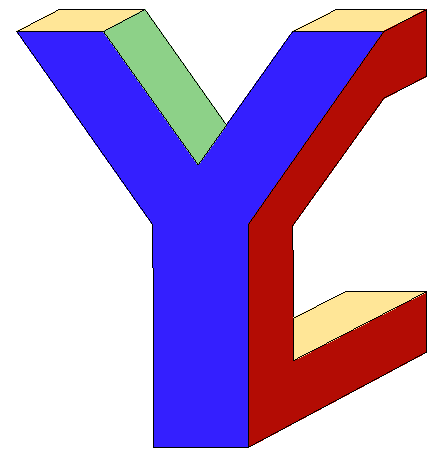
\includegraphics[height=1.5cm]{pictures/YC_logo.pdf}
        \end{center}
        &
        \begin{center}
            
\includegraphics[height=1.5cm]{pictures/SPbGU_Logo.png}
        \end{center} 
    \end{tabular}
	\titlepage
\end{frame}



%\begin{frame}
%	\begin{center} 
%		{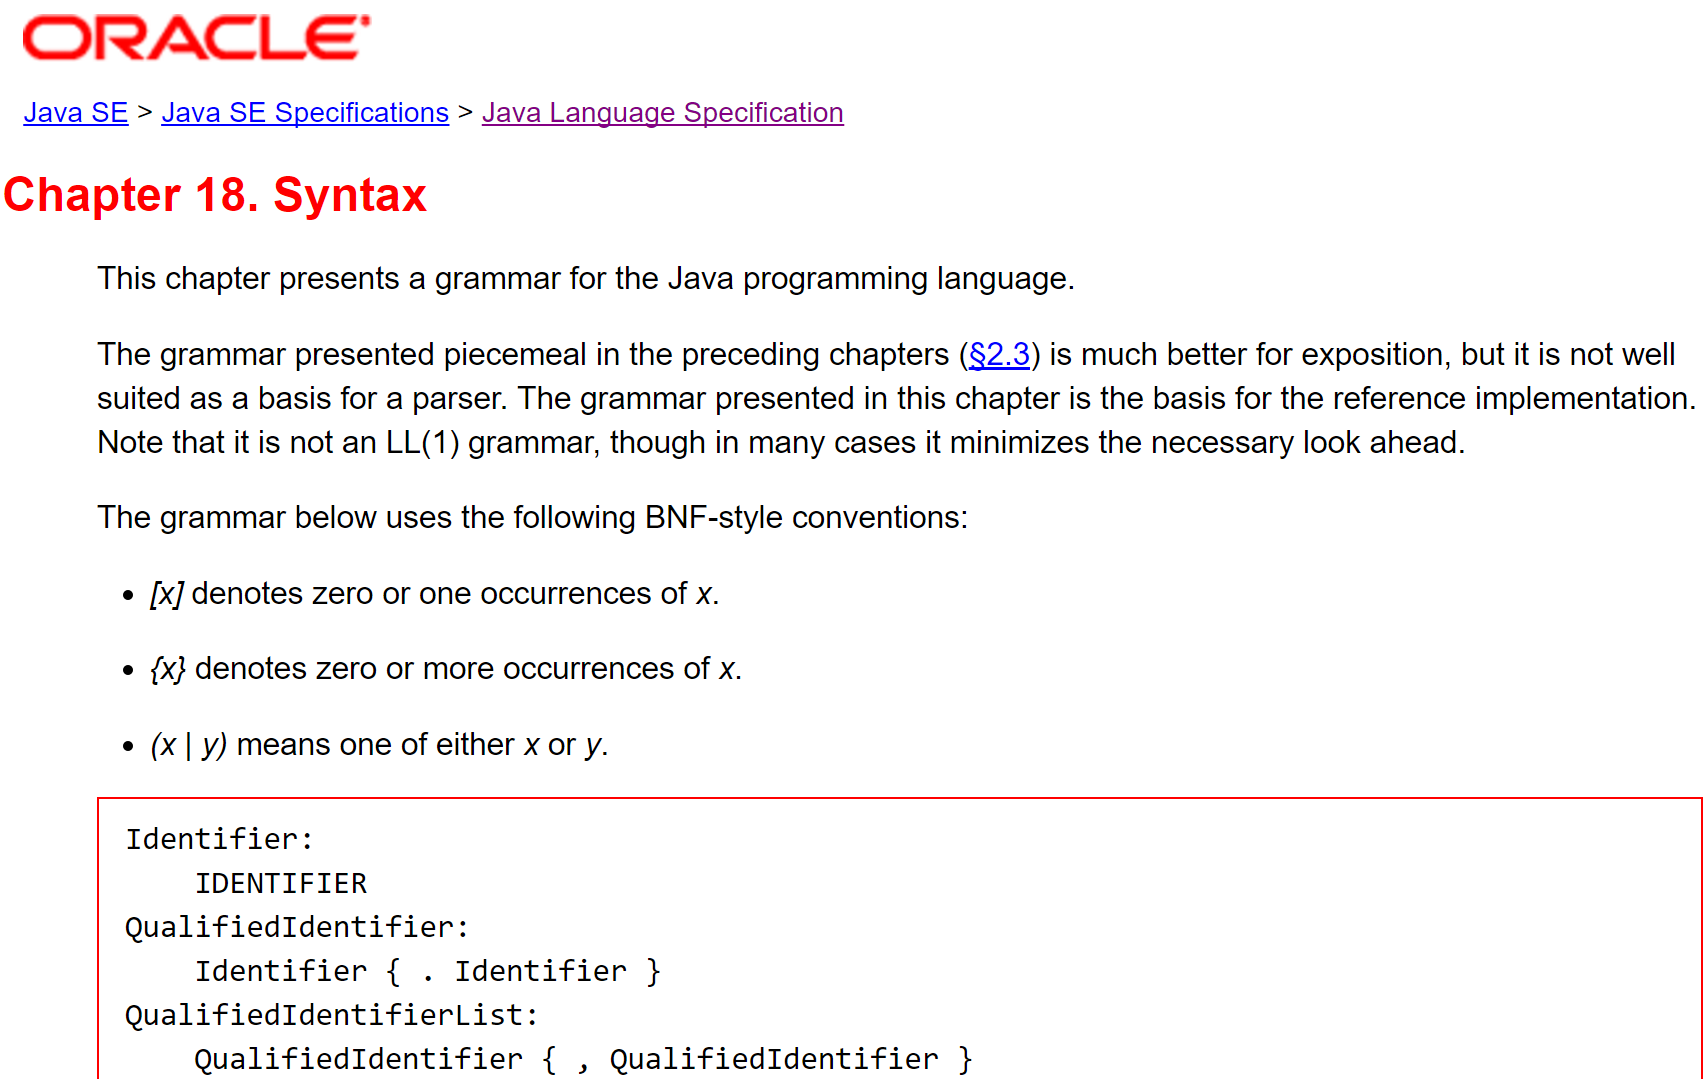
\includegraphics[width=12cm]{pictures/java_grammar.png}} 
%	\end{center}
%\end{frame}
\begin{frame}
     \frametitle{Shuffled Languages}
     \only<1>{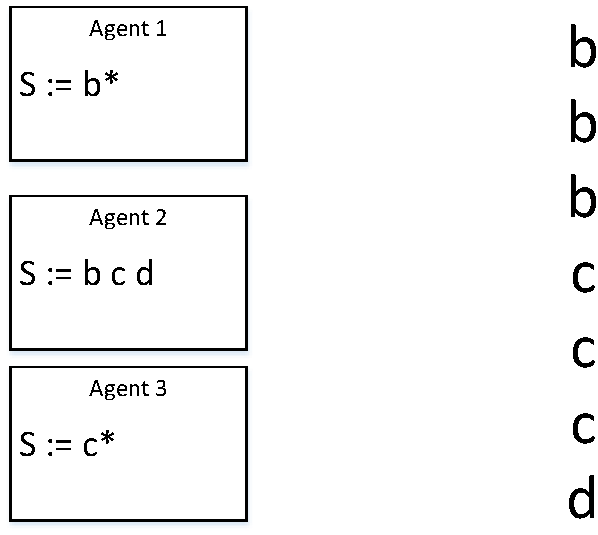
\includegraphics[width=8cm]{pictures/agents.pdf}}
     \only<2-3>{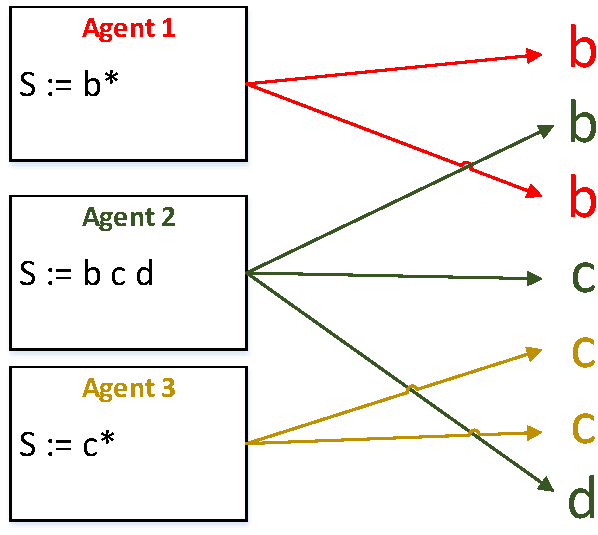
\includegraphics[width=8cm]{pictures/agentsColored.pdf}}
     
     \only<3>{\textbf{Проблема:} Грамматик может быть очень много, а задача NP-полная}
 \end{frame}
 
 \begin{frame}
     \frametitle{Существующие подходы}
         \begin{itemize}
             \item (Maraist, 2016) Generalized LR parsing and the shuffle operator 
             \item Используется GLR
             \item Во время разбора отслеживаются позиции сразу во всех грамматиках
             \item Пространство поиска сужается за счёт поддержания наиболее вероятных веток разбора
             \item Не строятся деревья разбора
         \end{itemize}
 \end{frame}
 
 \begin{frame}
     \frametitle{Наш подход}
     \begin{center}
         синтаксический анализ графов  +  метод ветвей и границ
     \end{center}
 \end{frame}
 
 
 \begin{frame}
     \frametitle{Анализ графов}
     \begin{itemize}
         \item Выделяем все возможные подпоследовательности из входа и обрабатываем как пути в графе
         \only<1>{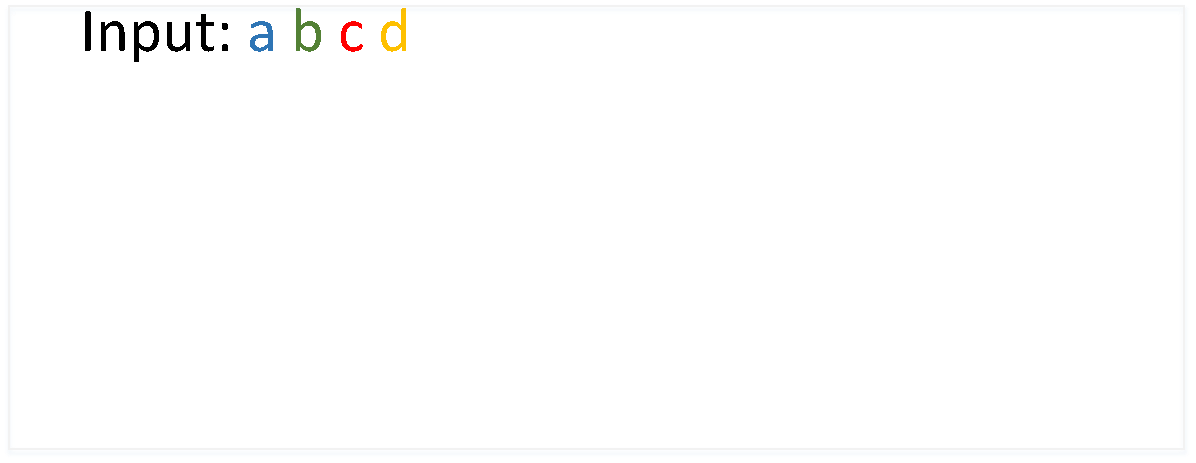
\includegraphics[width=11cm]{pictures/inputAsGraph1.pdf}}
         \only<2>{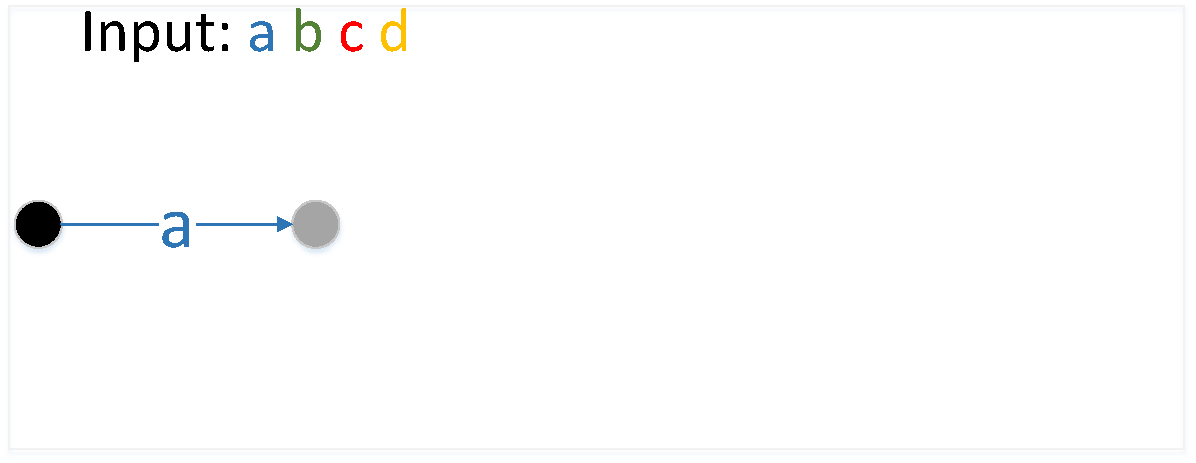
\includegraphics[width=11cm]{pictures/inputAsGraph2.pdf}}
         \only<3>{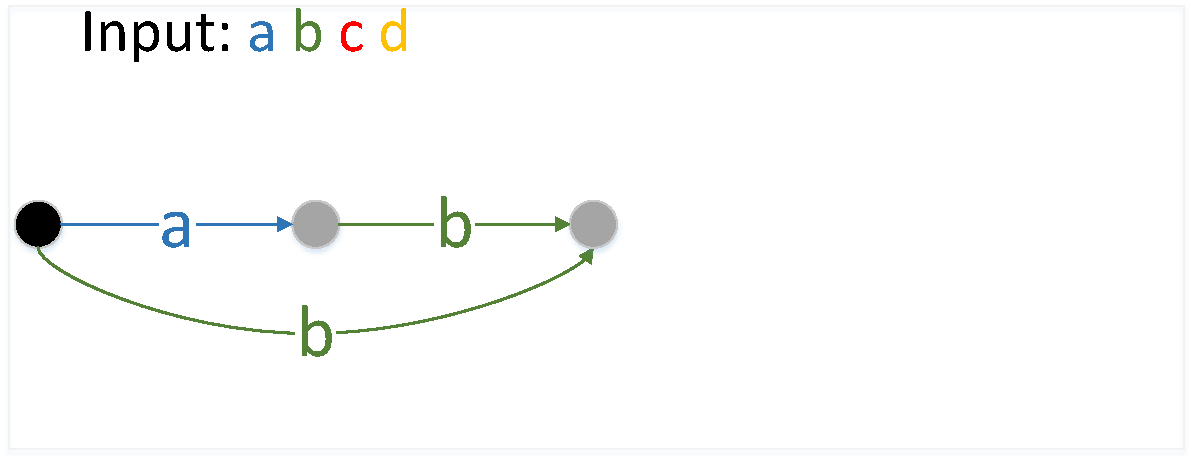
\includegraphics[width=11cm]{pictures/inputAsGraph3.pdf}}
         \only<4>{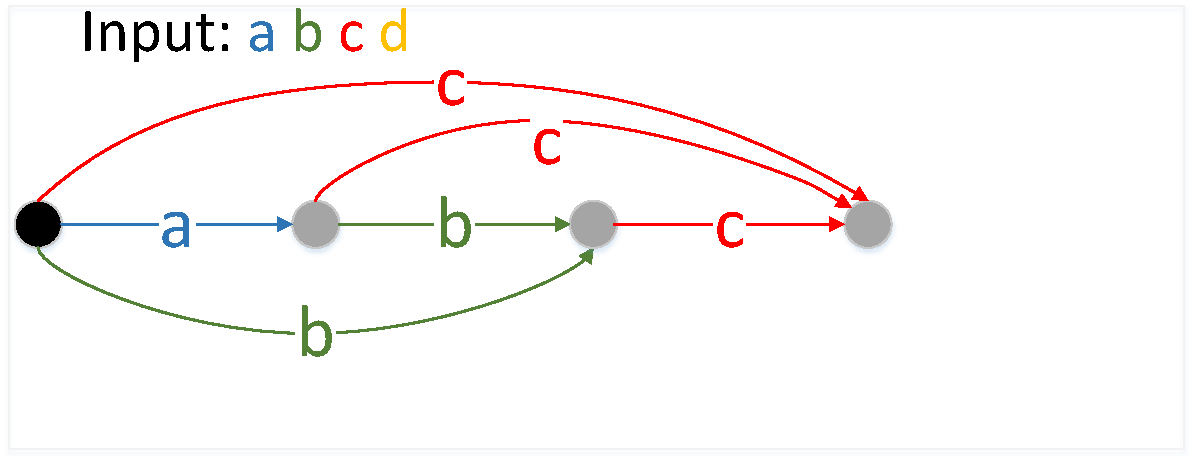
\includegraphics[width=11cm]{pictures/inputAsGraph4.pdf}}
         \only<5->{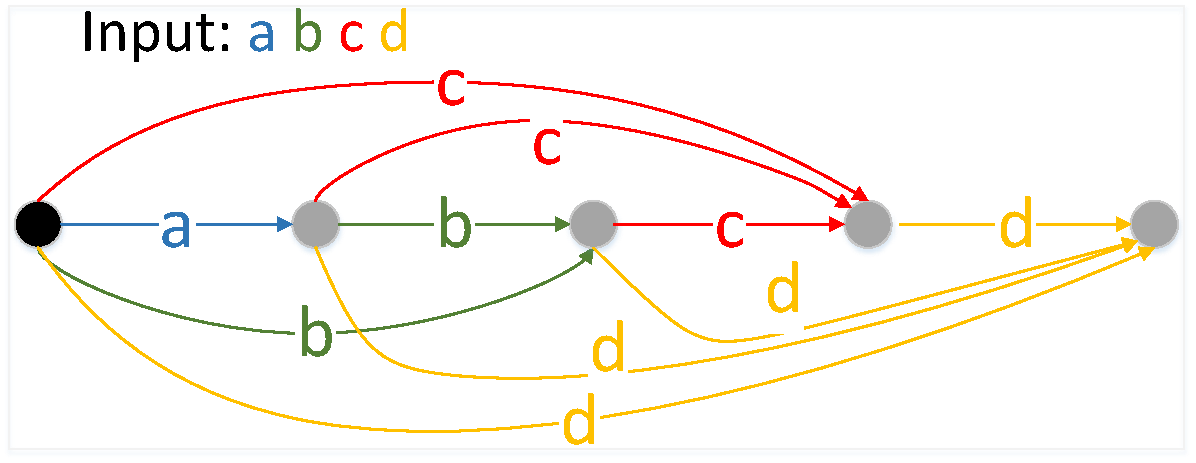
\includegraphics[width=11cm]{pictures/inputAsGraph5.pdf}}
         \only<6->{\item Для каждой грамматики анализ производится независимо --- можно распараллелить}
         \only<7>{\item Результат --- лес разбора всех подпоследовательностей для каждой грамматики}
     \end{itemize}
 \end{frame}
 
 \begin{frame}
	\frametitle{Метод ветвей и границ}
	\begin{itemize}
		\item Восстанавливаем входную последовательность по лесам разбора
        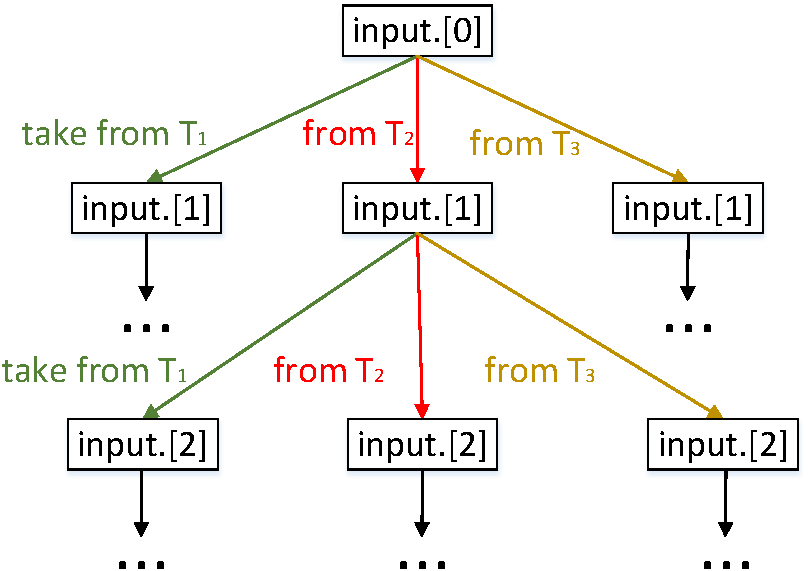
\includegraphics[width=10cm]{pictures/BnBtree.pdf}
	\end{itemize}
\end{frame}


 \begin{frame}
    \frametitle{Пример восстановления входа}
    \begin{center}
        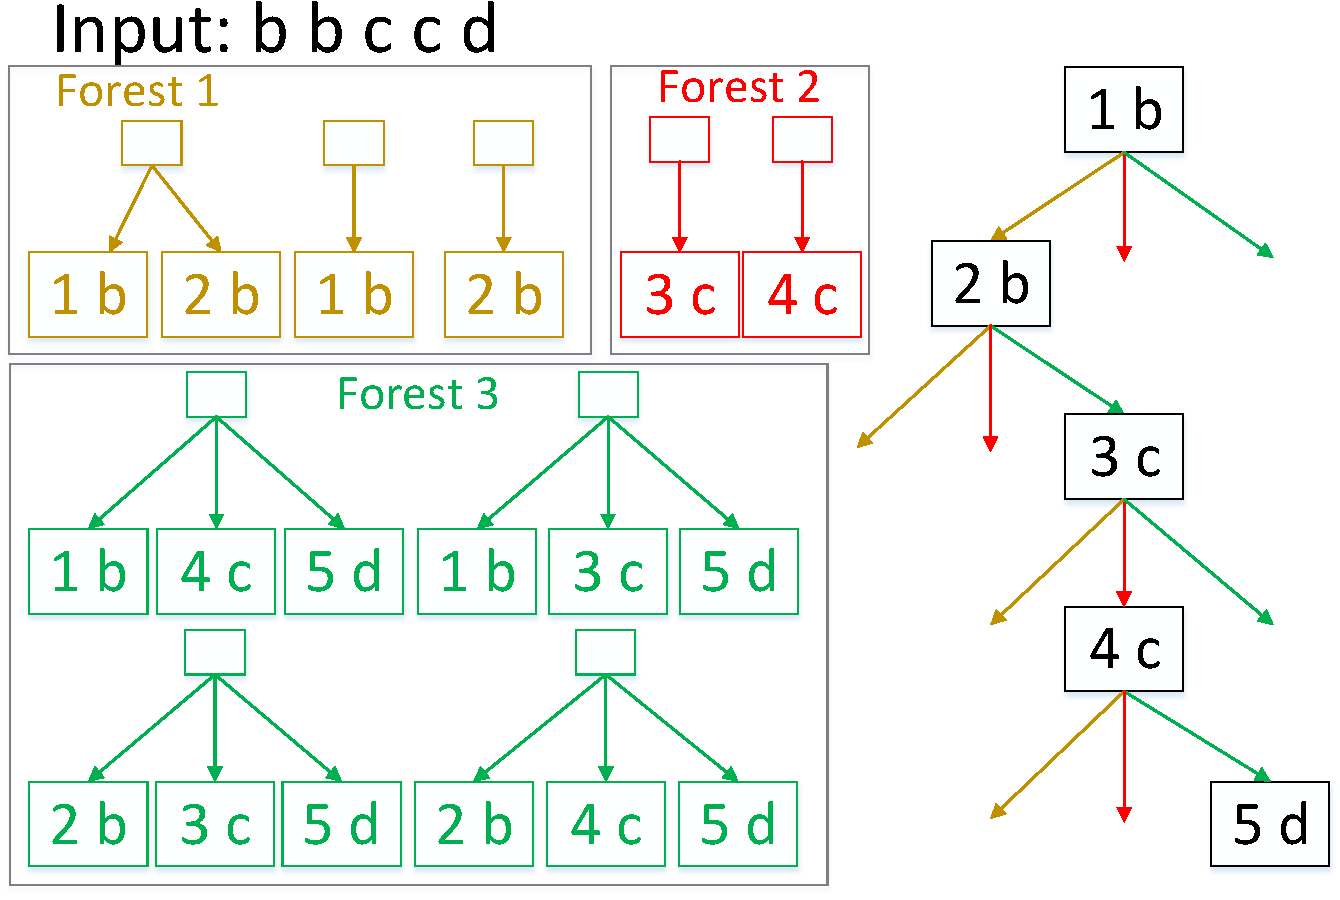
\includegraphics[width=9.5cm]{pictures/BnBexample.pdf}
    \end{center}
    \begin{itemize}
        \item Отсечение ветви если невозможно взять токен из данного леса
        \item Различные ветки обрабатываются независимо --- можно распараллелить
        \item Можно выбирать наиболее вероятную ветку
    \end{itemize}
\end{frame}

 \begin{frame}
    \frametitle{Прогресс работы}
    \begin{itemize}
        \item В поисках данных для адекватного тестирования и сравнения
        \item Планируется публикация результатов
    \end{itemize}
\end{frame}
\end{document}